
\documentclass{article}
\usepackage[latin1]{inputenc}
\usepackage{tikz}
\usetikzlibrary{shapes,arrows}
\usetikzlibrary{backgrounds}


%tikystzles
\tikzstyle{normal} = [rectangle, thick, minimum width=2.0cm, minimum height=1cm,text centered, draw=black]
\tikzstyle{grey} = [rectangle, thick, minimum width=2.0cm, minimum height=1cm,text centered, draw=black, fill=black!20]

\tikzstyle{arrow} = [thick,->,>=stealth]


\begin{document}
\begin{center}
	

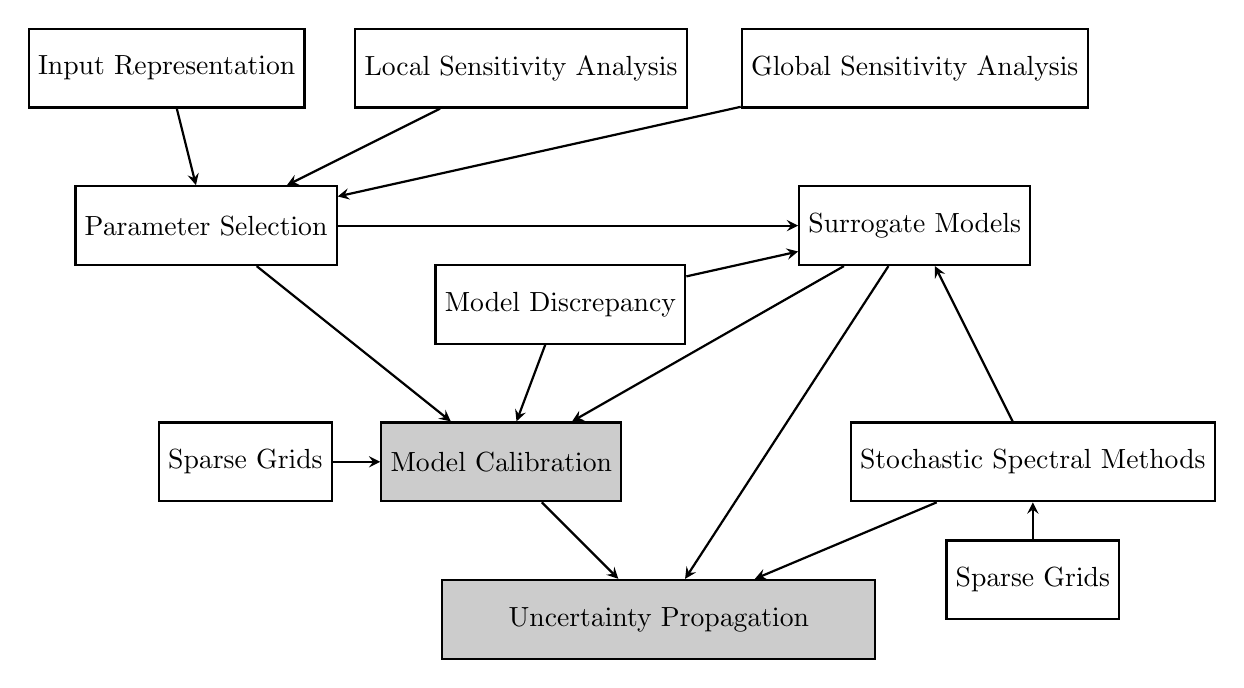
\begin{tikzpicture}[node distance=2cm]
% nodes
\node (ir) [normal] {Input Representation};
\node (lsa) [normal, right of=ir, xshift=2.5cm] {Local Sensitivity Analysis};
\node (gsa) [normal, right of=lsa, xshift=3.0cm] {Global Sensitivity Analysis};

\node (ps) [normal, below of=ir, xshift=0.5cm] {Parameter Selection};
\node (md) [normal, right of=ps, xshift=2.5cm, yshift=-1.0cm] {Model Discrepancy};
\node (sm) [normal, right of=md, xshift=2.5cm, yshift=+1.0cm] {Surrogate Models};

\node (sg) [normal, below of=ps, xshift=0.5cm, yshift=-1.0cm] {Sparse Grids};
\node (mc) [grey, right of=sg, xshift=1.25cm] {Model Calibration};
\node (ssm) [normal, right of=mc, xshift=4.75cm] {Stochastic Spectral Methods};

\node (up) [grey, below of=mc, xshift=2.0cm, minimum width=5.5cm] {Uncertainty Propagation};
\node (sg2) [normal, below of=ssm, yshift=0.5cm] {Sparse Grids};

%edges
\draw [arrow] (ir) -- (ps);
\draw [arrow] (lsa) -- (ps);
\draw [arrow] (gsa) -- (ps);

\draw [arrow] (ps) -- (sm);
\draw [arrow] (md) -- (sm);
\draw [arrow] (ssm) -- (sm);

\draw [arrow] (ps) -- (mc);
\draw [arrow] (md) -- (mc);

\draw [arrow] (sg) -- (mc);
\draw [arrow] (sm) -- (up);
\draw [arrow] (sg2) -- (ssm);

\draw [arrow] (mc) -- (up);
\draw [arrow] (ssm) -- (up);

% Background Edge. DOES NOT WORK
\begin{scope}[on background layer]

\draw [arrow] (sm) -- (mc);

\end{scope}





\end{tikzpicture}
\end{center}
\end{document}